\documentclass[11pt, oneside]{article} 
\usepackage{geometry}
\geometry{letterpaper} 
\usepackage{graphicx}
	
\usepackage{amssymb}
\usepackage{amsmath}
\usepackage{parskip}
\usepackage{color}
\usepackage{hyperref}

\graphicspath{{/Users/telliott_admin/Dropbox/Tex/png/}}
% \begin{center} 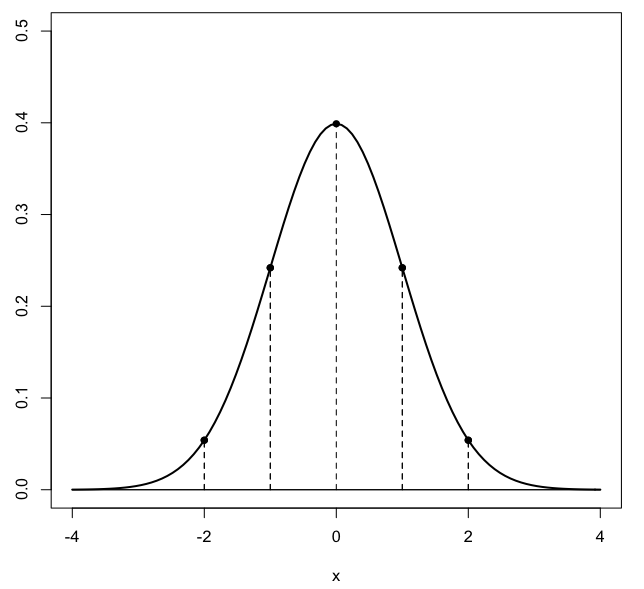
\includegraphics [scale=0.4] {gauss3.png} \end{center}

\title{Real numbers}
\date{}

\begin{document}
\maketitle
\Large

\subsection*{unit square}

It seemed at first that a perfectly consistent system of mathematics could be built up out of only the rational numbers.  However, it was discovered that some "numbers" cannot be represented by a rational number $p/q$ with integer $p$ and $q$.

Probably the simplest example is to consider a unit square and its diagonal.  The unit square has sides of length $1$ and Pythagoras tells us that the length of the diagonal is $\sqrt{1^2 + 1^2} = \sqrt{2}$.

Clearly, this is a valid physical length (just draw the diagonal, then transfer it to the number line).

Yet as you probably know, we cannot solve the equation $(p/q)^2 = 2$ for integer $p$ and $q$ (that is, rational number $p/q$).

And generally, many numbers (defined as solutions to equations like $r^2 = 2$ or $r^2 = 3$) cannot be represented by a rational number $p/q$ with integer $p$ and $q$.  

Despite the density of the rational numbers --- recall the infinite number of rational numbers in the interval $[0,1]$, nevertheless there are values that cannot be represented as rational numbers.  This situation is described by saying that the rational number line has "holes" in it.

\subsection*{no holes}

We introduce the concept of the real numbers $\mathbb{R}$ to include all the numbers we know so far: the natural numbers, the integers, the rational numbers $p/q \in \mathbb{Q}$, \emph{plus} the irrational numbers like $\sqrt{2}$ and also $\pi$ and $e$.  In this section, when we talk about real numbers we are really exploring the properties of those real numbers which are not rational, the set $- \mathbb{Q}$. 

The discovery that one cannot find integer $p$ and $q$ such that
\[ (\frac{p}{q})^2 = 2 \]
is due to the Pythagorean school and was most unwelcome since it screwed up their cherished theory of the universe.

The standard proof is by contradiction.  We suppose that $p$ and $q$ exist with this property.  Crucially, if $p$ and $q$ have a common factor we can certainly remove it by division, so that we must start with $p/q$ already in lowest terms.

An elegant way to state this is to use the theorem which says that each number has a unique prime \emph{factorization}.  For example:
\[ 12 = 2 \times 2 \times 3 \]
\[ 256 = 2 \times 2 \times 2 \times 2 \times 2 \times 2 \times 2 \times 2 \]
\[ 4841 = 47 \times 103 \]
So for any $p$ and $q$ if they have a common factor it is certain that we can find it, and remove it by division.

Another important preliminary result is that the square of an even number is an even number.

\textbf{Proof}:  every (positive) even number can be expressed as $n = 2k, \ k \in \mathbb{N}$, and then

\[ n^2 = (2k)^2 = 4k^2 = 2 \cdot 2 k^2 = 2m \]
is even.  On the other hand, every (positive) odd number has an odd square because it has the form $n = 2k + 1, \ k \in \mathbb{N}$ so

\[ n^2 = (2k + 1)^2 = 2 \ [ \ 2 \cdot (k^2 + k) \ ] \  + 1 = 2m + 1 \]
and so is odd.

Returning to
\[ (\frac{p}{q})^2 = \frac{p^2}{q^2} = 2 \]
A simple rearrangement 
\[ p^2 = 2 q^2 \]
shows that $p^2$ must be even, and from the above argument, $p$ must be even.  Rewrite $p = 2p'$.  Then

\[ \frac{(2p')^2}{q^2} = 2 \]

\[ 4 p'^2 = 2 q^2 \]
\[ 2 p'^2 = q^2 \]
Hence $q^2$ is even and so is $q$, which contradicts the assumption of $p$ and $q$ as having no common factors.  

This proves that integer $p$ and $q$ with the property $p/q = \sqrt{2}$ cannot be found.

\subsection*{alternative proof}
This is such an important result that we discuss another proof of it, following Stewart and Tall's \emph{The Foundations of Mathematics}.  It uses the prime factorization theorem from above.  

\textbf{Euclid's lemma} says that if a prime $p$ divides the product of two integers $a$ and $b$, then $p$ must divide at least one of $a$ and $b$.

It's a bit convoluted to prove so we will assume that part.  

From Euclid's lemma we obtain the Fundamental Theorem of arithmetic, also called the unique factorization theorem.  This says that every integer larger than 1 is either prime or is a unique product of prime factors.

Suppose $s > 1$ is the product of prime factors in two different ways:
\[ p = p_1 \cdot p_2 \dots \]
\[ q = q_1 \cdot q_2 \dots \]

By Euclid's lemma, $p_1$ must divide one of $q_1$ etc.  But these are all prime.  Therefore $p_1$ equals one of the $q_i$, say $q_1$.  Thus
\[ \frac{p}{p_1} = p_2 \dots \]
\[ \frac{p}{q_1} = q_2 \dots \]

This can be done for each of the factors $p_i$.  Therefore the factorization is unique.

Unique prime factorization can be used in turn to prove that $\sqrt{2}$ is irrational.  Since every integer $p$ is a product $p_1 p_2 \dots$, and every rational number $p/q$ is
\[ \frac{p_1 \cdot p_2 \dots}{q_1 \cdot q_2 \dots} \]
where no $p_i$ equals any $q_i$.

Every rational number squared is 
\[ \frac{p_1^2 \cdot p_2^2 \dots}{q_1^2 \cdot q_2^2 \dots} \]

But $2$ has only itself as a factor and that factor only occurs once.  There is no rational number with this property.

\end{document}